\documentclass[11pt]{article}
\usepackage[utf8]{inputenc}
\usepackage[T1]{fontenc}
\usepackage{amsmath}
\usepackage{amsfonts}
\usepackage{amssymb}
\usepackage[version=4]{mhchem}
\usepackage{stmaryrd}
\usepackage{graphicx}
\usepackage[export]{adjustbox}
\graphicspath{ {./images/} }

\begin{document}
Co-Investments

\section*{Overview of Co-Investing}
In recent years, asset owners have increasingly directly invested in companies or alongside main PE funds in the form of co-investments. Some LPs generally look for such opportunities and even ask for co-investment rights. But co-investing differs from being an LP in a blind pool fund and therefore requires additional knowledge and skills.

As noted by Greene and Rigdon (2016), ${ }^{1}$ Greene, D., and A. Rigdon (2016), Private Equity Co-Investment, in Tom Alabaster, Global Investment Funds: A Practical Guide to Structuring, Raising and Managing Funds, Globe Law \& Business Ltd. co-investment typically involves one or more LPs of the main fund being invited by the GP to invest in one or more of the portfolio companies through a "sponsor-controlled investment vehicle typically a limited partnership or limited liability company." However, in addition to co-investing in a partnership controlled by the GP of the main fund, co-investing also occurs through three other vehicles. Three alternative co-investing structures involve: ${ }^{2}$ Ibid. (1) the LP invests directly into one or more of the portfolio companies of the main fund; (2) one or more LPs use a GP-controlled fund created apart from the main fund for the purposes of investing in one or more of the same portfolio companies selected for the main fund; and (3) making investments in co-investment programs in which the specific investments are identified and decisions on whether to co-invest are made on an ongoing and deal-bydeal basis.

The second investing structure discussed above is a top-up fund. A top-up fund is used to co-invest in one or more future investments of the main fund. An annex fund is used to co-invest in one or more pre-existing investments. ${ }^{3}$ Ibid. Terms for co-investing are often described in detail in side letters between the GP and the investors participating in the co-investment. ${ }^{4}$ Ibid. These issues may include lock-step provisions. A lock-step provision in a co-investment agreement specifies that the terms and conditions of the co-investor-GP relationship is the same as the terms and conditions of the LP-GP relationship. Co-investments may be performed in the context of bridge financing. In the context of private equity financing, bridging is when the GP makes an investment in the main fund while agreeing to sell that investment at a subsequent time to co-investors such that co-investors receive bridge-financing from the main fund between the time the investment is made and the time that the co-investor(s) takes ownership. Side letters are detailed in the Co-investments lesson Section 4.4, Evolution of Investing in Private Equity. From the LP perspective, an LP's primary view of co-investments is often as a way of enhancing their overall returns primarily from accessing a private company while paying lower management fees or carried interest charges than found in the main PE fund or potentially paying no management or carried interest fees. While GPs may charge low or no management fees for providing this access to co-investment opportunities, they may charge other fees such as transaction fees. To be able to go this low or no-fee, no-carried-interest route, the LP generally needs to be an existing investor in the GP's main fund. Further, co-investing opportunities may be linked to whether the LP has a good relationship with the GP or is able to offer expertise in a particular field.

On the other hand, there is also the emergence of funds that focus on co-investments as the co-investment concept matures. There are funds of funds that have a mix of co-investments and PE fund investments and multi-manager co-investment funds that focus exclusively on co-investments. These additional ways of accessing coinvestments focus more on return enhancement, and not so much on control and cost efficiency for the asset owners. The exhibit Different Ways an Asset Owner Can Access Co-Investments shows the different ways an asset owner can access co-investments.

\begin{center}
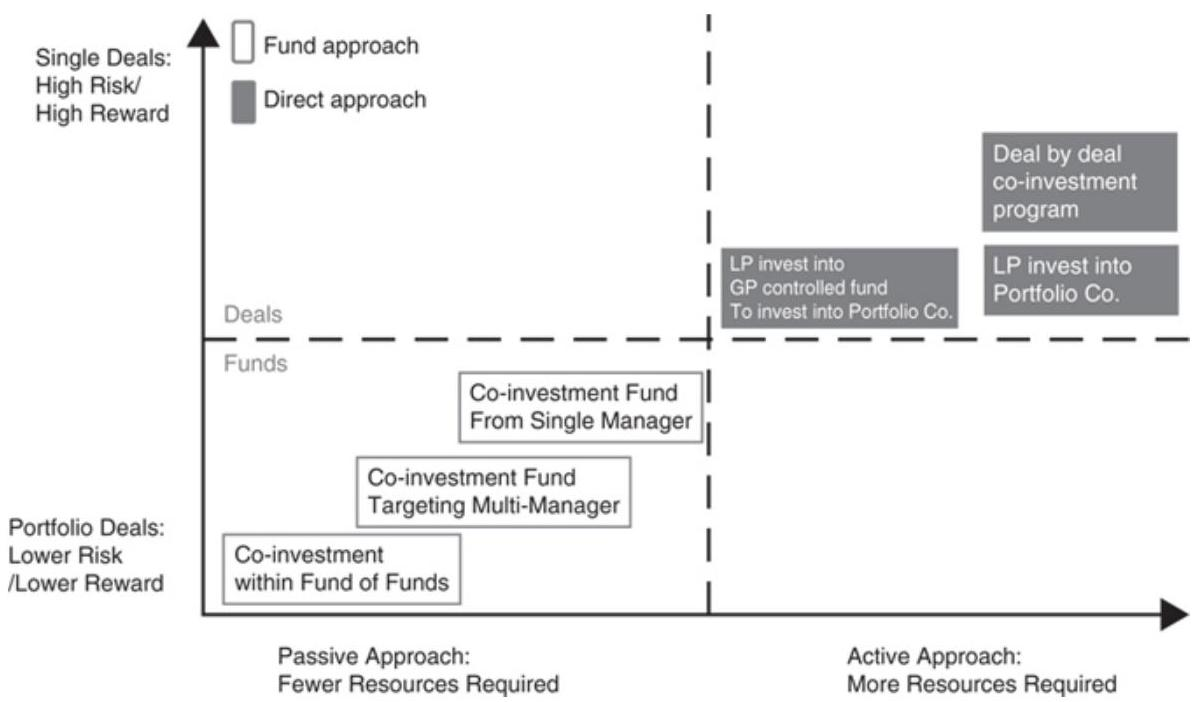
\includegraphics[max width=\textwidth]{2024_04_10_a087d40a569f64263ea7g-2}
\end{center}

\section*{Different Ways an Asset Owner Can Access Co-Investments}
Source: CAIA Association

From the GP perspective, ${ }^{5} \mathrm{Ibid}$. co-investment can increase the size of the fund and, potentially, the level of diversification. Co-investing can allow a manager to make larger investments without dedicating too much of the main fund's capital to a single transaction, which is why co-investments can increase the level of diversification within the main fund. Further, co-investing can provide financing that facilitates the transition from one partnership to a successor partnership when the GP has not been able to arrange sufficient financing yet to launch a main fund.

Finally, not all co-investment deals come without fees and carried interest. Some LPs co-invest by paying promote rather than carried interest. In the context of private equity, promote is a fee based on profits that is similar to carried interest but is typically associated with more specific duties such as the creation and marketing of a specific investment opportunity. The fees for co-investment deals vary according to the nature of the deal. A GP typically asks for more fees if they sourced the deal and are expected to do as much work for the co-investment as for their fund. Through industry surveys and various studies, there are three main fee structures for co-investments:

\begin{itemize}
  \item No fees. $0 \%$ annual management fee. $0 \%$ carried interest.
  \item $1 \%$ annual management fee. $10 \%$ carried interest.
  \item $0 \%$ annual management fee. $20 \%$ carried interest.
\end{itemize}

\section*{Investment Processes for Co-Investing}
There is no set universal model for co-investments. The main differences between co-investing and direct investing include how the investments in the portfolio companies are sourced and selected (in the main fund the sponsor makes the decisions and in co-investing the LPs tend to be able to pick which investments they help fund). However, generally, opportunities are deals that the fund manager has prescreened, selected, structured, and priced. The exhibit Comparison of CoInvestment, Fund Investment, And Solo Investment shows the differences in investment process for fund investing, co-investment, and solo investment. The following points summarize the co-investment processes:

\begin{itemize}
  \item Portfolio strategies of LPs typically include a reserve of between $10 \%$ and $20 \%$ to be allocated to co-investments. Many investors do not appear to have a specific allocation and tend to do co-investments on an opportunistic basis, but a PE investment program requires a critical mass for being able to pursue coinvestments.
  \item The sponsor of the main fund generally organizes the co-investment for the LPs. The GP usually needs a significant number of primary fund commitments to generate a meaningful co-investment deal flow. LPs need to express their interest in co-investments at the time of the fund commitment and reinforce this through regular follow-up calls and meetings.
  \item Importantly, the efficient execution of the process, whether turning a deal down quickly or working in parallel with and at the same pace as the GP, is critical to successful co-investing.
  \item Co-investing requires a different skill set than does main fund investing, as LPs need to have much greater insight into individual deals. Even if they are unable to form a view on the attractiveness of individual investments, they may still be attracted by potential savings on management fees and carried interest.
\end{itemize}

For smaller LPs, the fact that an occasionally too-high minimum amount is required for co-investments can cause problems. In such situations, the opportunity for co-investing may have to be passed up, especially if the amount required for co-investing is close to the amount the small institution originally committed to a fund. One way of overcoming this is to approach other investors and do the co-investment alongside them.

Co-investing can be viewed as a way to overcome some of the restrictions of investing in the main limited partnership structure. However, co-investing is not a panacea and clearly is not for the risk-averse or inexperienced PE investor.

\begin{center}
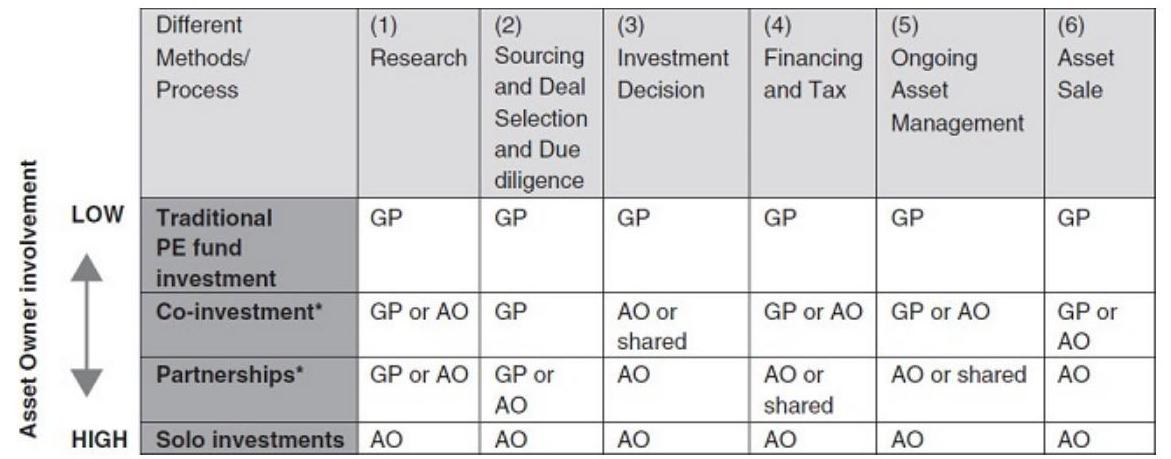
\includegraphics[max width=\textwidth]{2024_04_10_a087d40a569f64263ea7g-4}
\end{center}

Comparison of Co-Investment, Fund Investment, And Solo Investment

${ }^{*}$ Different Asset Owners may have varying involvement than summarized in the exhibit.

Source: CAIA Association. Shaded row indicates the typical co-investment structure.

\section*{Potential Advantages of Co-Investing}
In addition to avoiding the double layer of management fees, co-investing potentially offers the LP a number of potential advantages:

\begin{itemize}
  \item Superior returns: Theoretically, co-investing offers enhanced returns by reducing fees and increasing exposure to portfolio companies selected by the LP for their potential upside.
  \item Targeted investment tool: Commitments to PE funds are a relatively blunt allocation tool. Co-investments are a tool for building a targeted allocation to specific investments. If an LP follows the policy of co-investment only in portfolio companies that are already profitable or that would reach profitability soon, this could, for example, mitigate the exposure to cash-burning startups. Also, it may be difficult to find funds that specifically target, say, eco-innovation, but it is very likely that a number of funds have one or another company active in this sector in their portfolios. Co-investing allows the LP to tilt the portfolio balance in a desired direction or to fill specific target allocations in the LP's portfolio.
  \item Better management of portfolio diversification: Co-investments can mitigate an institutional portfolio of funds' overdiversification or overexposure. Coinvestments provide flexibility to capitalize on industry-specific and country-specific opportunities as they arise. They may also be an answer to funds with liquidity management problems and can be a meaningful strategy with a first-time team, serving as a tool to assist fund managers in the execution of transactions. In the context of an overcommitment strategy, prospective co-investment opportunities allow an LP not to execute the option if the liquidity is insufficient to honor the resulting increase in capital calls. Moreover, it could be used for managing foreign exchange risks, as usual hedging products would be too uneconomical for PE funds, with their long lifetimes and volatile cash flows.
  \item Mitigating dilution: For investments in small funds, co-investments also improve downside protection, as they mitigate the dilution of a fund's shareholding when available resources are insufficient for follow-on investing. This can be attractive when funds lack sufficient capital for follow-on investment (particularly in a venture context), allowing them to boost their firepower on certain deals without resorting to collaboration with other GPs, which can potentially lead to conflicts and rivalry. However, if disputes on an investment arise, relationships with LPs and future fundraisings can be negatively affected.
  \item Dual level of review for investments: The institutional investor can leave the difficult work of deal sourcing and assessment to experienced industry experts. Even though LPs need to do some due diligence, they can save significant time, because much of the screening is done by fund managers, as is a large degree of the time-consuming task of monitoring.
  \item Improved monitoring: As an indirect benefit, a co-investment allows for improved monitoring of the funds and a further reduction of the information asymmetry between fund managers and their investors. It can help LPs better understand the investment process and environment, allowing for better fund selections and reinvestment decisions. The information co-investors receive is quite important because it gives an idea about how the fund managers operate and often goes beyond the standard reporting LPs usually receive.
  \item Establishing relationships to invitation-only funds: For LPs who face problems getting access to top funds, co-investments form an important part of a strategy that helps to land slots in a handful of sought-after funds. Moreover, an LP can benefit from the investment skills of such funds even if not yet invested and get access to transactions of top-tier PE firms.
  \item Reduction of the J-curve effect: Co-investments, like secondaries, are viewed as leading to a reduction of the J-curve effect and improved capital deployment and returns. Smoothing the cash-flow J-curve (that is, the concentrations in outflows due to capital calls during the early years of an investment program) may make sense in some situations but will be difficult to achieve, as there is usually too little and too inconsistent quality deal flow to have a meaningful impact on sizable portfolios.
\end{itemize}

Importantly, co-investing conforms to the important characteristics of real options and can maximize a fund investment's upside by increasing the exposure to the best-performing portfolio companies. However, it is definitely not a guarantee for higher returns in the asset class and, in fact, is often seen as quite difficult to execute.

\section*{Potential Expected Disadvantages of Co-Investing}
Indeed, there are also disadvantages to take into consideration when engaging in co-investments:

\begin{itemize}
  \item Unbalanced portfolios: Because an LP's participation in co-investing may build up additional exposure to certain companies, industries, or geographies, risks can increase very specifically with regard to individual portfolio companies. If a few large co-investments are undertaken, there is also the danger of holding an overly concentrated portfolio of directly held investments.
  \item Increased fiduciary risk: For investment decisions taken outside a formal partnership structure, there is exposure to fiduciary risk. If things go wrong at the investment level, LPs may be exposed to legal liabilities and reputational risks.
  \item Conflicts of interest: There is a wide consensus that investors should focus on committing to the very best funds irrespective of co-investing rights or opportunities. Moreover, co-investing can become a source of conflicts of interest between LP investors in the same main fund. Co-investing LPs may be given preference to their specific investments even if this is detrimental to the main fund's performance.
  \item Disagreements among LPs: Problems associated with failing co-investments can become complicated when one company with several co-investing LPs goes bankrupt, leading to disagreements between the parties involved. Also, fund managers may be inclined to spend more time on particular portfolio companies if they receive additional management fees or carried interest, or if the co-investing LP is of strategic importance for them.
  \item Allocation of fees: Co-investing can increase the potentially serious issue of the allocation of expenses between the GP, the LPs of the main fund, and the coinvestors. Fee allocation is receiving increasing attention as an issue tied to inherent conflicts of interest between the parties to private equity investments.
\end{itemize}

\end{document}